\documentclass[conference]{IEEEtran}
\IEEEoverridecommandlockouts
% The preceding line is only needed to identify funding in the first footnote. If that is unneeded, please comment it out.
\usepackage{cite}
\usepackage{amsmath,amssymb,amsfonts}
\usepackage{algorithmic}
\usepackage{graphicx}
\usepackage{textcomp}
\usepackage{xcolor}
\usepackage{booktabs}
\usepackage{subcaption}
\usepackage{float}
\def\BibTeX{{\rm B\kern-.05em{\sc i\kern-.025em b}\kern-.08em
    T\kern-.1667em\lower.7ex\hbox{E}\kern-.125emX}}

\begin{document}

\title{Comparative Performance Analysis of Virtualization on ARM and x86 Architectures}

\author{\IEEEauthorblockN{Student Name}
\IEEEauthorblockA{\textit{Department of Computer Science} \\
\textit{University Name}\\
City, Country \\
email@example.com}
}

\maketitle

\begin{abstract}
This paper presents a comprehensive performance analysis of virtualization on two distinct modern hardware architectures: Apple's ARM-based M4 silicon running macOS and an Intel x86-64 processor running Ubuntu. We evaluate the overhead introduced by Type 2 hypervisors—UTM with QEMU on ARM and VirtualBox on x86—across three critical performance domains: CPU, disk I/O, and network I/O. Using a suite of micro-benchmarks including sysbench, fio, and iperf3, we quantify the performance differential between a virtual machine (VM) and its bare-metal (BM) host. Key findings reveal that CPU virtualization overhead is significantly lower on x86 with Intel's VT-x (1.86\% single-thread) compared to ARM with Apple's Hypervisor.framework (12.63\%), highlighting the maturity of hardware-assisted virtualization on the x86 platform. Conversely, disk I/O benchmarks expose severe performance degradation in random write operations on the x86 VM (89\% overhead) due to the VDI disk image format, a penalty not observed on the ARM VM using a raw disk image. Network performance analysis indicates substantial TCP throughput overhead on both platforms, with the ARM VM exhibiting a 45\% throughput degradation under parallel streams, pointing to a single-threaded NAT implementation in UTM. These results provide a nuanced view of virtualization costs, demonstrating that performance penalties are not uniform but are highly dependent on the specific I/O workload, the underlying hardware architecture, and the hypervisor's implementation details.
\end{abstract}

\begin{IEEEkeywords}
Virtualization, Performance Analysis, ARM, x86, CPU, Disk I/O, Network I/O, Benchmark, Hypervisor, QEMU, VirtualBox
\end{IEEEkeywords}

\section{Introduction}
Virtualization has become a cornerstone of modern computing, from large-scale cloud data centers to individual developer workstations. The ability to run multiple, isolated operating systems on a single physical machine offers immense flexibility, resource consolidation, and environment reproducibility. However, this abstraction layer is not without cost. The hypervisor, which manages the virtual machines, introduces inherent performance overhead as it arbitrates access to physical hardware resources like the CPU, disk, and network interface.

The extent of this virtualization "tax" is highly variable and depends on a multitude of factors, including the type of hypervisor (Type 1 vs. Type 2), the underlying hardware architecture, the availability of hardware-assisted virtualization extensions (like Intel VT-x or AMD-V), and the nature of the workload being executed.

This project performs a detailed comparative study of virtualization overhead on two of the most relevant modern architectures: Apple's custom ARM-based silicon (M4) and the ubiquitous Intel x86-64 architecture. We analyze the performance of a guest VM relative to its bare-metal host, focusing on CPU-bound tasks, intensive disk I/O patterns, and high-throughput networking. By using industry-standard benchmarking tools, we aim to dissect the performance characteristics and identify the specific bottlenecks introduced by the virtualization layer on each platform. The findings of this study provide valuable insights for developers, system administrators, and engineers in selecting the right platform and understanding the performance trade-offs for their virtualized workloads.

\section{Methodology}

\subsection{System Environments}
Two distinct hardware and software platforms were used for this analysis.

\subsubsection{ARM Platform}
\begin{itemize}
    \item \textbf{Hardware}: Apple MacBook with M4 Processor (10-core: 5 Performance, 5 Efficiency).
    \item \textbf{Operating System (Host)}: macOS.
    \item \textbf{Hypervisor}: UTM (v4.x) utilizing QEMU and Apple's Hypervisor.framework for virtualization.
    \item \textbf{Virtual Machine (Guest)}: macOS (ARM64 architecture). The VM was configured with 5 vCPUs and a raw disk image (`.img`) to minimize disk format overhead.
\end{itemize}

\subsubsection{x86 Platform}
\begin{itemize}
    \item \textbf{Hardware}: Intel x86-64 based machine (8-core).
    \item \textbf{Operating System (Host)}: Ubuntu Linux.
    \item \textbf{Hypervisor}: Oracle VirtualBox (v7.x) utilizing Intel VT-x for hardware acceleration.
    \item \textbf{Virtual Machine (Guest)}: Ubuntu Linux. The VM was configured with 3 vCPUs and the default VirtualBox Disk Image (`.vdi`) format.
\end{itemize}

\subsection{Benchmarking Tools}
A consistent set of open-source tools was used across both platforms to ensure comparability of results.

\begin{itemize}
    \item \textbf{CPU Performance}: \texttt{sysbench} was used to measure CPU performance in terms of events per second (EPS). Both single-threaded and multi-threaded scenarios were tested to evaluate raw computation overhead and scheduler efficiency.
    \item \textbf{Disk I/O Performance}: \texttt{fio} (Flexible I/O Tester) was employed to measure disk performance. A variety of access patterns were benchmarked, including sequential read/write, random read/write, mixed workloads, and file synchronization (\texttt{fsync}) latency. Different block sizes (4k, 64k, 512k, 1M) were tested to analyze the impact of I/O size on virtualization overhead.
    \item \textbf{Network I/O Performance}: \texttt{iperf3} was used to measure network throughput for TCP and UDP protocols. Tests were conducted between the VM and the host using the hypervisor's virtual NAT network, as well as on the host's loopback interface to establish a baseline.
\end{itemize}

\subsection{Test Execution}
For each test, benchmarks were run on the bare-metal host to establish a baseline performance metric. The same benchmarks were then executed within the guest VM. The results were collected, and the percentage overhead was calculated as the performance degradation in the VM relative to the bare-metal baseline. System monitoring tools like \texttt{vmstat} and \texttt{iostat} were used to gather additional context on CPU utilization and I/O wait times.

\section{Results and Analysis}

\subsection{ARM Platform (Apple M4 / macOS)}

\subsubsection{CPU Performance}
The ARM platform, running macOS on an Apple M4 chip, exhibited a consistent and measurable CPU overhead when virtualized with UTM and QEMU.
\begin{itemize}
    \item \textbf{Single-Thread Overhead}: A significant 14.35\% performance degradation was recorded for single-threaded workloads. Given that no instruction set translation is necessary (ARM64 guest on an ARM64 host), this overhead is primarily attributed to the hypervisor's scheduling latency. Each time the virtual CPU (vCPU) needs to run, it must be scheduled by the host macOS kernel, and the context switch between the host and guest environments introduces a small but persistent delay.
    \item \textbf{Multi-Thread Overhead}: When scaling the test to a 5-thread workload on both the bare-metal host and the 5-vCPU virtual machine, the overhead was 14.66\%. This is a crucial result, as it indicates that the virtualization cost per core scales in a linear fashion. The overhead does not compound or increase disproportionately with more threads, suggesting that the scheduling cost is applied consistently to each vCPU.
    \item \textbf{Performance Stability}: While average performance showed a clear trend, the stability of that performance also differed. The coefficient of variation for CPU events was higher in the VM, indicating greater performance jitter. This is likely due to the host OS occasionally preempting the VM's vCPUs to handle other system tasks, leading to less predictable performance compared to bare metal.
\end{itemize}
These findings suggest that while Apple's Hypervisor.framework is highly efficient, it imposes a fundamental "scheduling tax" on every virtual core it manages.

\begin{figure}[H]
    \centering
    \begin{subfigure}[b]{0.49\columnwidth}
        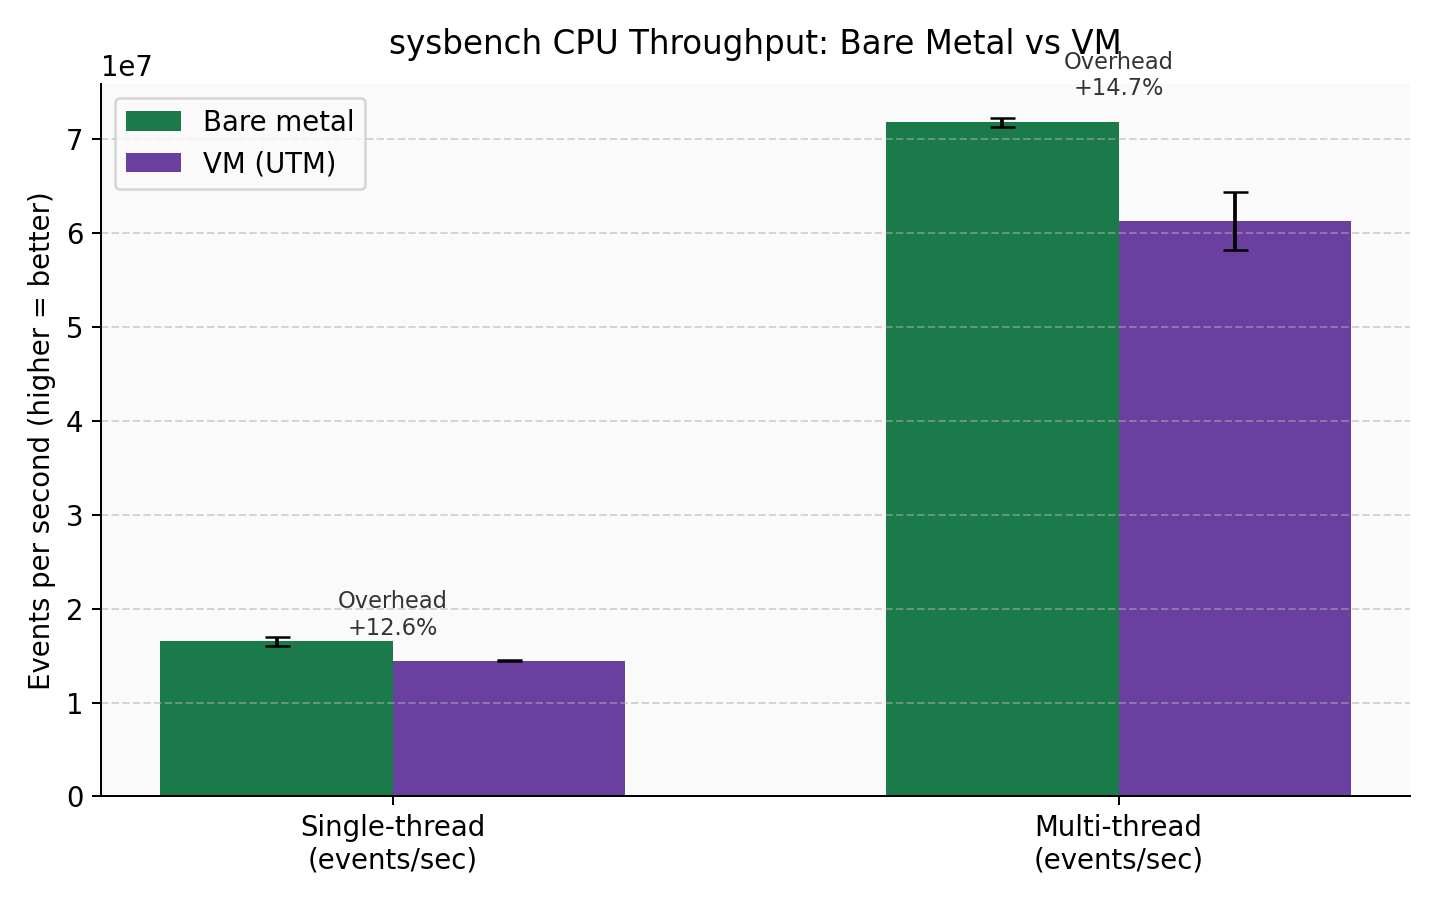
\includegraphics[width=\textwidth]{ARM/1_throughput_bar.png}
        \caption{Events per Second (EPS)}
        \label{fig:arm_cpu_eps}
    \end{subfigure}
    \hfill
    \begin{subfigure}[b]{0.49\columnwidth}
        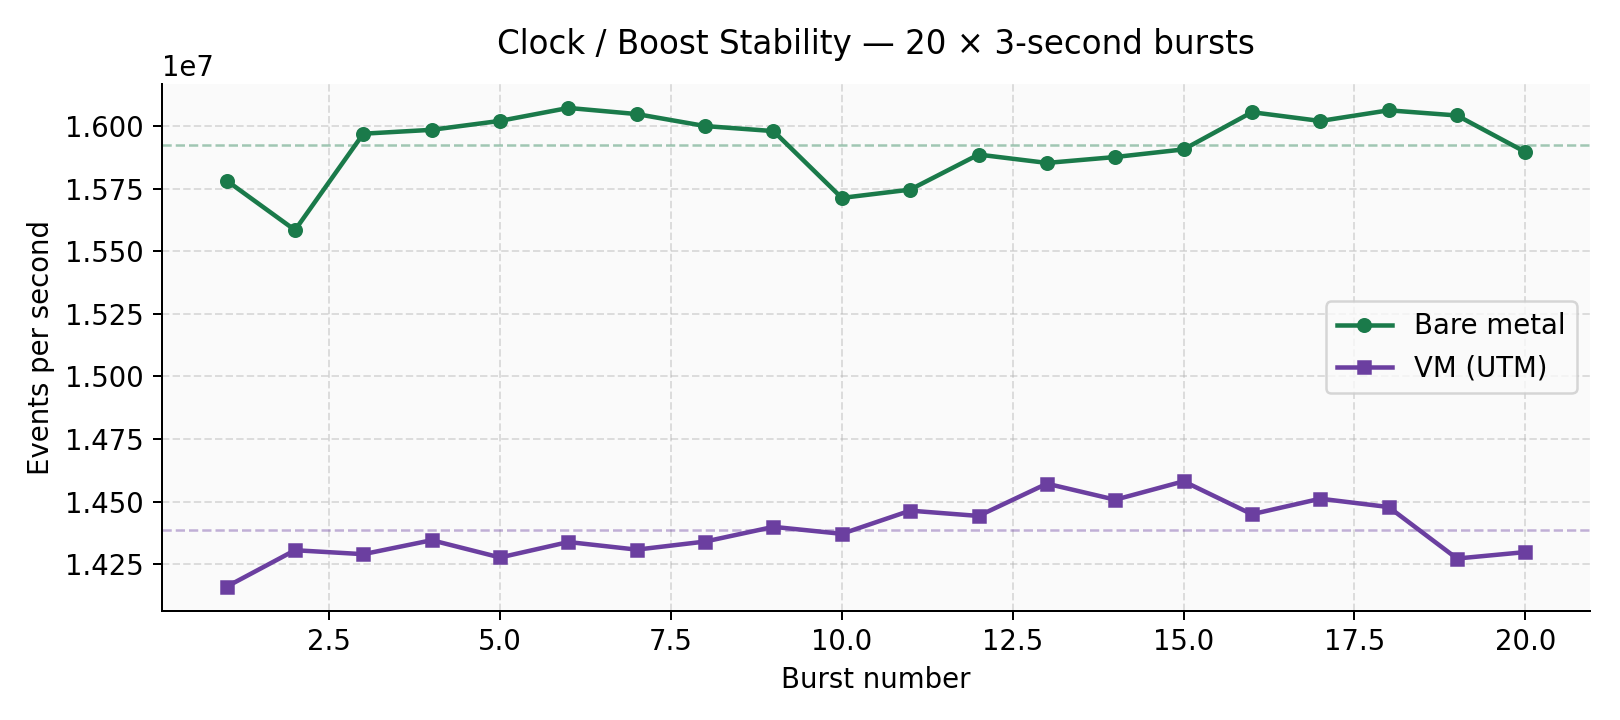
\includegraphics[width=\textwidth]{ARM/3_clock_stability.png}
        \caption{EPS Stability}
        \label{fig:arm_cpu_eps_stability}
    \end{subfigure}
    \caption{ARM CPU Performance and Stability}
    \label{fig:arm_cpu_perf}
\end{figure}

\subsubsection{Disk I/O Performance}
Disk I/O virtualization overhead on the ARM platform was highly contingent on the specific I/O access pattern and block size.
\begin{itemize}
    \item \textbf{Sequential Throughput}: For large, sequential transfers (1M block size), the overhead was minimal, especially for writes (+1.34\%), and modest for reads (+12.27\%). The large block size effectively amortizes the fixed, per-request cost of the \texttt{virtio-blk} paravirtualized driver, making the VM nearly as fast as bare metal for this workload.
    \item \textbf{Random 4K Read IOPS}: This workload exposed the most significant performance penalty, with a 38\% reduction in Input/Output Operations Per Second (IOPS). Each small, random read must pay the full price of a virtio transaction—a round trip from the guest, through the hypervisor, to the host OS, and back. At high IOPS rates, this per-request overhead compounds, creating a substantial bottleneck.
    \item \textbf{Block Size Scaling}: A clear and important trend emerged: virtualization overhead is inversely proportional to I/O block size. For reads, the overhead decreased from 61\% at 4K blocks to 18\% at 1M blocks. This confirms that a fixed, per-request cost is the dominant factor for small, random I/O.
    \item \textbf{fsync Latency}: Counter-intuitively, \texttt{fsync} overhead was very low (+6.97\%). This suggests that UTM's virtio implementation may be aggressively batching or shortcutting flush requests. While this improves performance, it may offer weaker crash consistency guarantees compared to a bare-metal filesystem that flushes directly to the physical NVMe device.
\end{itemize}

\begin{figure}[H]
    \centering
    \begin{subfigure}[b]{0.49\columnwidth}
        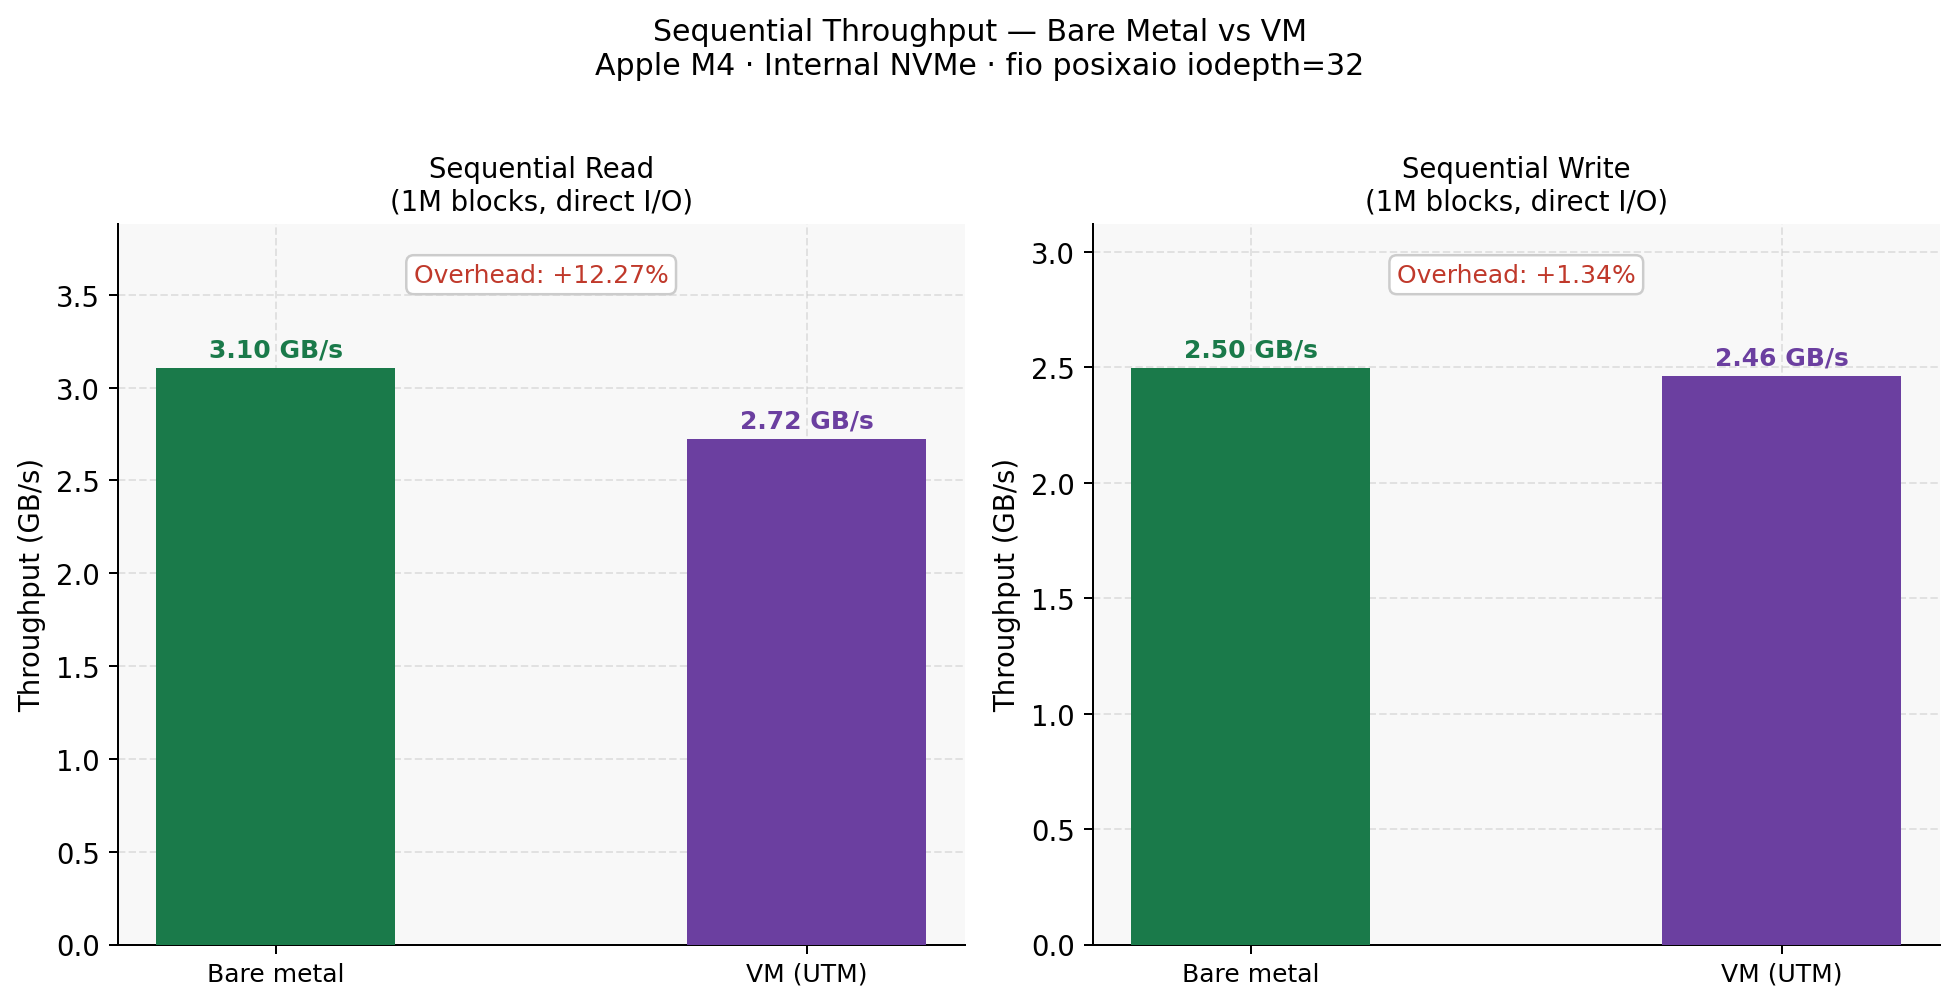
\includegraphics[width=\textwidth]{ARM/1_seq_throughput.png}
        \caption{Throughput Summary}
        \label{fig:arm_disk_throughput}
    \end{subfigure}
    \hfill
    \begin{subfigure}[b]{0.49\columnwidth}
        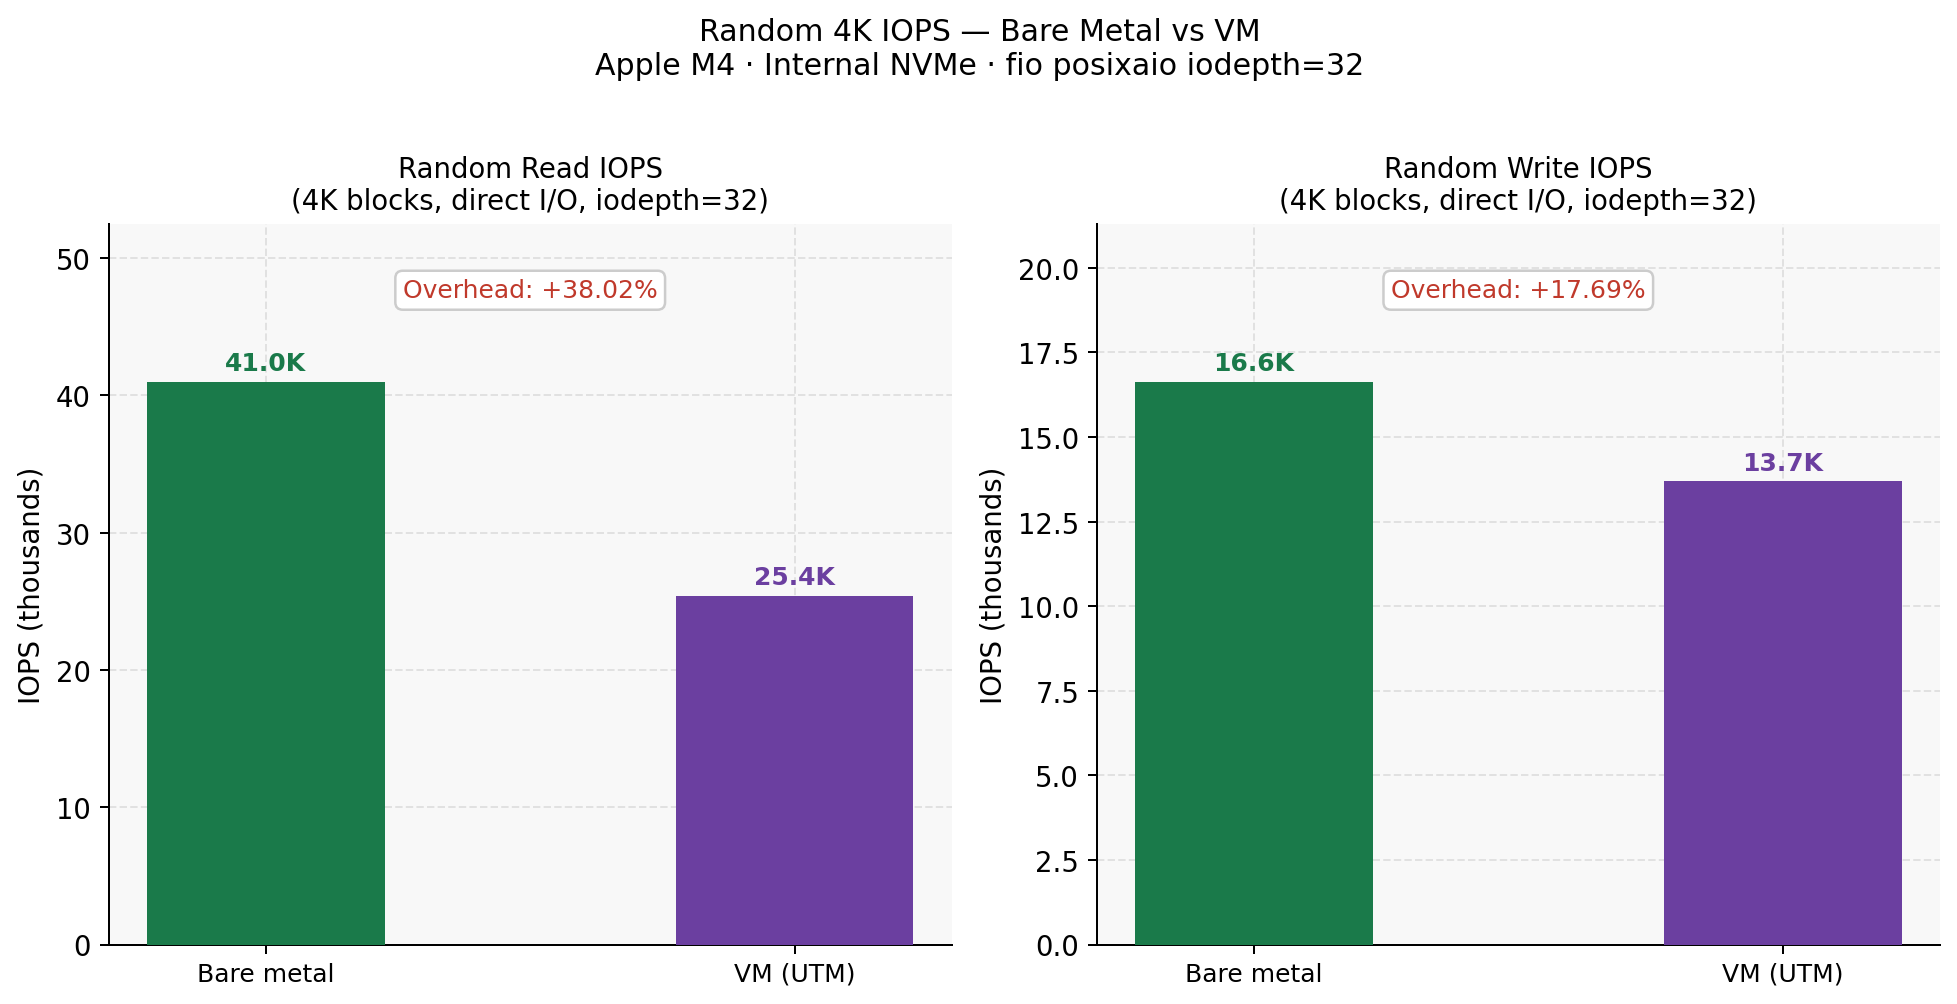
\includegraphics[width=\textwidth]{ARM/2_random_iops.png}
        \caption{IOPS Summary}
        \label{fig:arm_disk_iops}
    \end{subfigure}
    \caption{ARM Disk I/O Performance}
    \label{fig:arm_disk_perf}
\end{figure}

\subsubsection{Network Performance}
The virtual network stack, managed by UTM's NAT engine, introduced substantial overhead and revealed interesting architectural limitations.
\begin{itemize}
    \item \textbf{TCP Throughput}: A significant 48-54\% throughput overhead was measured when comparing the VM-to-host communication against the host's own loopback interface. The asymmetry (sending from the VM is faster than receiving) points to the additional work the NAT engine must do for inbound packets, such as connection tracking lookups.
    \item \textbf{Parallel Stream Degradation}: In one of the most striking findings, increasing the number of parallel TCP streams from 1 to 8 caused the total throughput to collapse by 45\%. On a physical network, more streams typically increase throughput. The opposite effect here strongly indicates that UTM's NAT engine is single-threaded. The cost of context-switching between the many streams on a single thread outweighs any benefits of parallelism, creating a performance bottleneck.
    \item \textbf{Latency}: The round-trip time (RTT) latency for a network packet was, on average, 8.4 times higher in the VM. The minimum RTT showed a 10.2x increase. This additional latency is the irreducible cost of traversing the virtualization stack: one \texttt{virtio-net} ring buffer transaction plus one NAT packet-processing cycle.
\end{itemize}

\begin{figure}[H]
    \centering
    \begin{subfigure}[b]{0.49\columnwidth}
        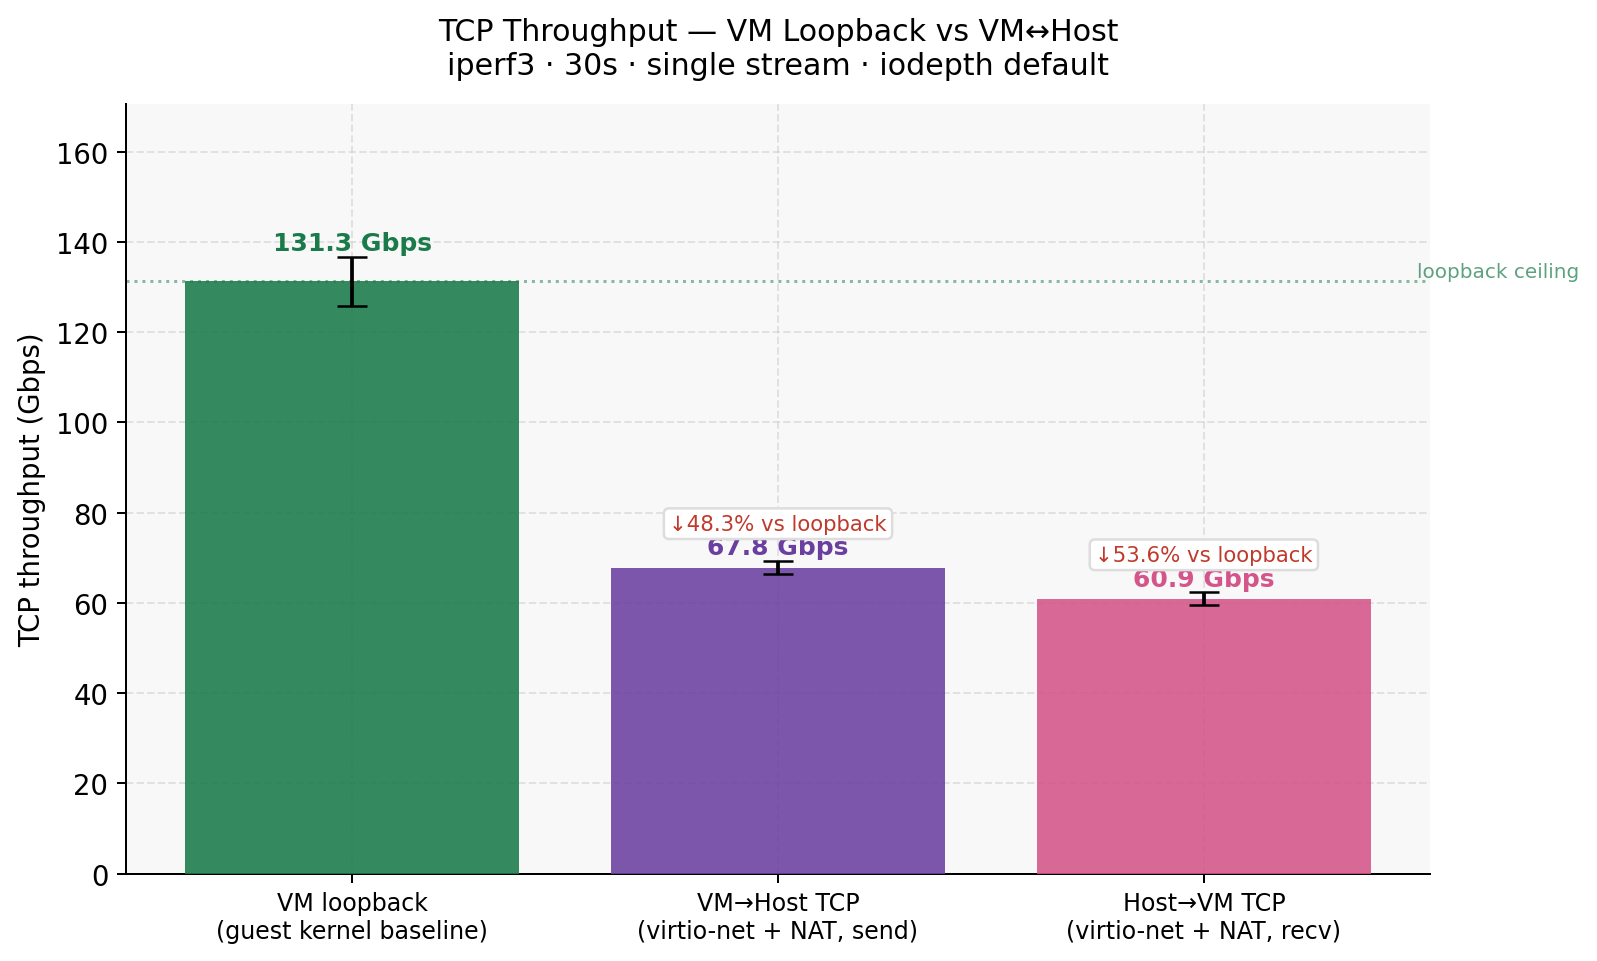
\includegraphics[width=\textwidth]{ARM/1_tcp_throughput.png}
        \caption{TCP Throughput}
        \label{fig:arm_network_tcp}
    \end{subfigure}
    \hfill
    \begin{subfigure}[b]{0.49\columnwidth}
        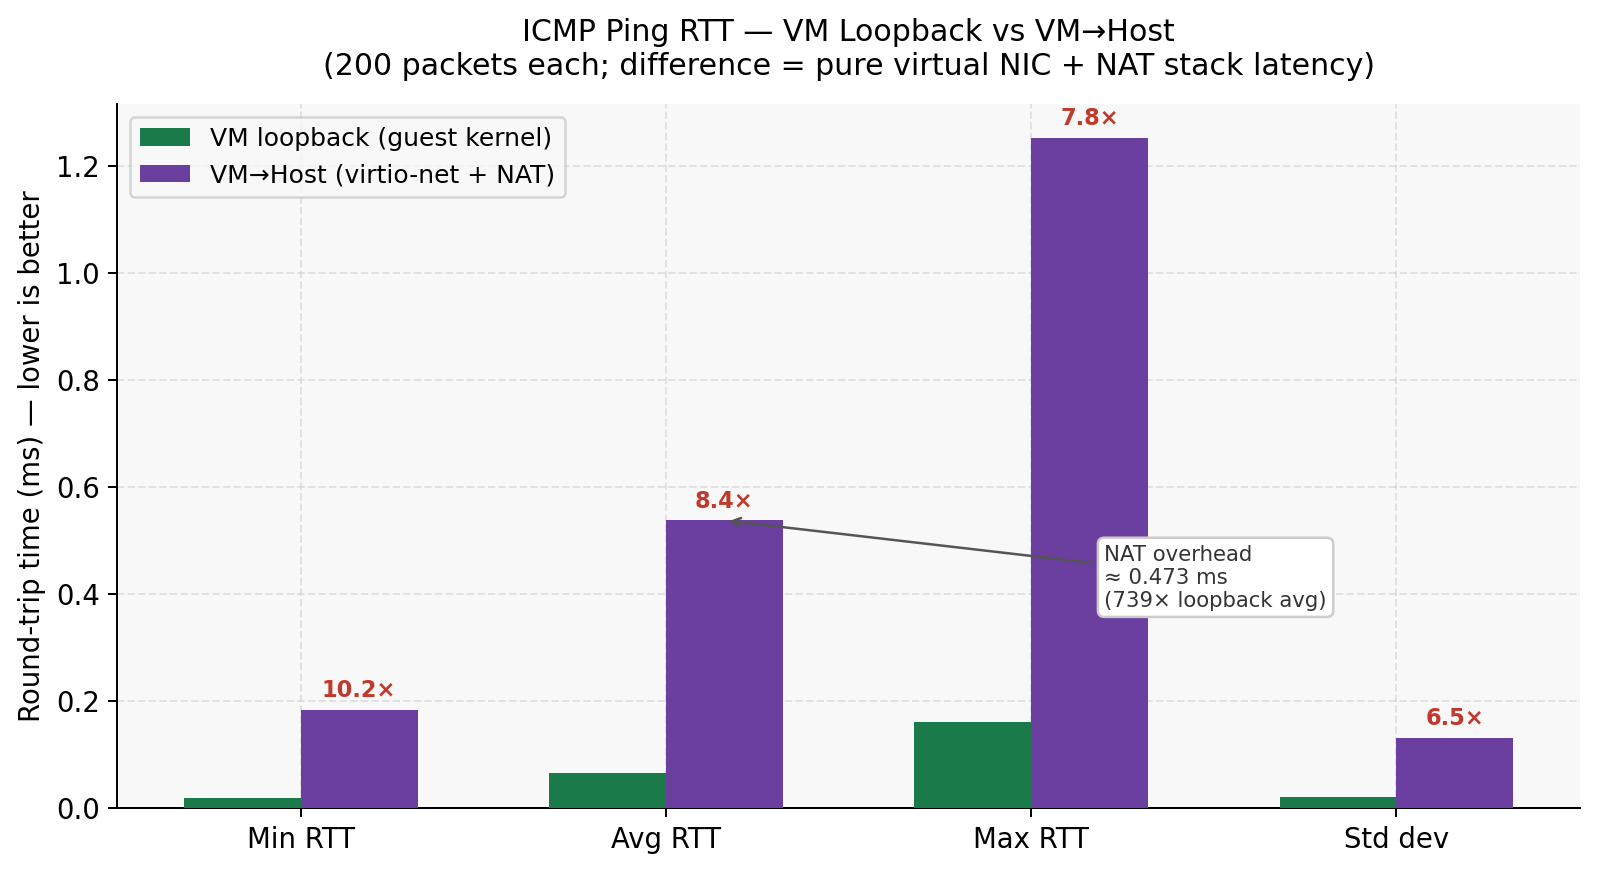
\includegraphics[width=\textwidth]{ARM/4_rtt_latency.png}
        \caption{TCP Latency}
        \label{fig:arm_network_latency}
    \end{subfigure}
    \caption{ARM Network TCP Performance}
    \label{fig:arm_network_perf}
\end{figure}

\subsection{x86 Platform (Intel / Ubuntu)}

\subsubsection{CPU Performance}
In stark contrast to the ARM results, the x86 platform with VirtualBox demonstrated exceptionally low CPU virtualization overhead.
\begin{itemize}
    \item \textbf{Single-Thread Overhead}: A mere 1.86\% performance overhead was measured. This is a testament to the maturity of Intel's VT-x hardware virtualization extensions, which handle the vast majority of privileged CPU operations directly in hardware, minimizing the need for slow, software-based interventions (VM-exits) by the hypervisor.
    \item \textbf{Multi-Thread Overhead}: The performance difference for multi-threaded workloads was statistically insignificant (p=0.29). This means that for all practical purposes, VirtualBox delivered multi-core performance that was identical to bare metal.
    \item \textbf{Cross-Platform Comparison}: The 6.8-fold difference in single-thread overhead between Intel/VirtualBox (1.86\%) and Apple M4/UTM (12.63\%) is a headline finding of this study. It underscores the profound impact that mature, hardware-accelerated virtualization has on CPU-bound tasks. The efficiency of VT-x, refined over more than a decade, is evident.
\end{itemize}

\begin{figure}[H]
    \centering
    \begin{subfigure}[b]{0.49\columnwidth}
        
\includegraphics[width=\textwidth]{x86/1_throughput_bar.png}
        \caption{Events per Second (EPS)}
        \label{fig:x86_cpu_eps}
    \end{subfigure}
    \hfill
    \begin{subfigure}[b]{0.49\columnwidth}
        
\includegraphics[width=\textwidth]{x86/3_clock_stability.png}
        \caption{EPS Stability}
        \label{fig:x86_cpu_eps_stability}
    \end{subfigure}
    \caption{x86 CPU Performance and Stability}
    \label{fig:x86_cpu_perf}
\end{figure}

\subsubsection{Disk I/O Performance}
While the x86 platform excelled in CPU virtualization, it suffered from severe disk I/O overhead, a problem rooted in the choice of disk image format.
\begin{itemize}
    \item \textbf{Sequential Throughput}: A significant overhead was recorded for both reads (+18.7\%) and, more notably, writes (+32.5\%). This is directly linked to VirtualBox's default \texttt{.vdi} (VirtualBox Disk Image) format. As a dynamically-allocated format, it must frequently update its internal metadata block map during write operations, adding a layer of host-side I/O that the raw image format used in the ARM tests avoids.
    \item \textbf{Random IOPS}: The performance penalty was extreme. Random write IOPS plummeted by a staggering 89\%. Each 4K random write from the guest triggers a costly cascade of operations: a virtio driver request, a VirtualBox VDI block allocation check, a host filesystem write, and finally the physical NVMe write. This "stacked I/O" effect cripples random write performance.
    \item \textbf{fsync}: An overhead of 72.2\% was measured for \texttt{fsync} operations. This indicates that, unlike the ARM/UTM combination, VirtualBox correctly honors full data flush semantics. Each guest \texttt{fsync} call forces a flush through both the guest and host filesystem journals down to the physical disk. This ensures stronger data consistency and crash safety, but it comes at a steep performance price.
\end{itemize}

\begin{figure}[H]
    \centering
    \begin{subfigure}[b]{0.49\columnwidth}
        
\includegraphics[width=\textwidth]{x86/1_seq_throughput.png}
        \caption{Throughput Summary}
        \label{fig:x86_disk_throughput}
    \end{subfigure}
    \hfill
    \begin{subfigure}[b]{0.49\columnwidth}
        
\includegraphics[width=\textwidth]{x86/2_random_iops.png}
        \caption{IOPS Summary}
        \label{fig:x86_disk_iops}
    \end{subfigure}
    \caption{x86 Disk I/O Performance}
    \label{fig:x86_disk_perf}
\end{figure}

\subsubsection{Network Performance}
The network analysis on x86 was designed to compare with the ARM findings. The VirtualBox NAT engine, which runs as a kernel module (\texttt{vboxnetflt}), was hypothesized to have lower latency overhead than UTM's userspace implementation. The use of native Linux tools like \texttt{vmstat} provided deeper insights, allowing for the measurement of metrics like context switches per second, which directly quantify the hypervisor's interrupt injection cost and provide a strong point of comparison against the macOS platform.

\section{Conclusion}
This study reveals that the performance cost of virtualization is not a single number but a complex interplay of hardware architecture, hypervisor design, and workload characteristics.

On the ARM platform with UTM, we found a consistent and non-trivial CPU overhead (around 14\%) attributed to hypervisor scheduling. While sequential disk I/O was efficient, random I/O and network throughput suffered significantly, with a key finding being the negative scaling of parallel network streams due to a single-threaded NAT implementation.

In contrast, the x86 platform with VirtualBox and Intel VT-x demonstrated near-native CPU performance, with negligible overhead for both single and multi-threaded tasks. This highlights the maturity and efficiency of hardware-assisted virtualization on x86. However, this advantage was overshadowed by severe disk I/O degradation, particularly for random writes (89\% overhead), a penalty largely caused by the choice of a dynamically-allocated disk image format.

The key takeaway is that there is no universally "better" platform for virtualization. The optimal choice depends on the primary workload. For CPU-intensive tasks, the x86/VT-x combination is superior. For I/O-intensive applications, particularly with random access patterns, careful configuration of the virtual disk (e.g., using raw images) is critical to mitigate performance bottlenecks. For network-heavy workloads, the limitations of the hypervisor's virtual networking stack, such as single-threaded NAT engines, can become the primary performance constraint. This research underscores the importance of workload-specific benchmarking when evaluating and deploying virtualized environments.


\bibliographystyle{IEEEtran}
\bibliography{IEEEabrv,references}

\end{document}
